
%(BEGIN_QUESTION)
% Copyright 2009, Tony R. Kuphaldt, released under the Creative Commons Attribution License (v 1.0)
% This means you may do almost anything with this work of mine, so long as you give me proper credit

Read and outline the ``Exclusive Valve Sequencing'' subsection of the ``Split-Ranging'' section of the ``Control Valves'' chapter in your {\it Lessons In Industrial Instrumentation} textbook.  Note the page numbers where important illustrations, photographs, equations, tables, and other relevant details are found.  Prepare to thoughtfully discuss with your instructor and classmates the concepts and examples explored in this reading.

\underbar{file i04220}
%(END_QUESTION)





%(BEGIN_ANSWER)


%(END_ANSWER)





%(BEGIN_NOTES)

Exclusive split-ranging is when two control valves operate off the same signal, in such a way that they move in opposite directions but yet are never both open at the same time.  Useful for heating/cooling and acid/base neutralization applications, where you do not want both functions to simultaneously occur. 

\vskip 10pt

The following illustration graphically depicts this type of valve sequencing:

$$\includegraphics[width=15.5cm]{i04220x01.eps}$$





\vskip 20pt \vbox{\hrule \hbox{\strut \vrule{} {\bf Suggestions for Socratic discussion} \vrule} \hrule}

\begin{itemize}
\item{} Describe a practical application for {\it exclusive} split-ranging.
\end{itemize}





\vfil \eject

\noindent
{\bf Prep Quiz:}

Identify the style of valve sequencing represented by the following diagram:

$$\includegraphics[width=15.5cm]{i04220x01.eps}$$

\begin{itemize}
\item{} Exclusive
\vskip 5pt 
\item{} Complementary
\vskip 5pt 
\item{} Inclusive
\vskip 5pt 
\item{} Gratuitous
\vskip 5pt 
\item{} Progressive
\vskip 5pt 
\item{} Ostentatious
\end{itemize}



%INDEX% Reading assignment: Lessons In Industrial Instrumentation, split-ranging (exclusive)

%(END_NOTES)


